
% \documentclass[manuscript]{aastex}
\documentclass[12pt,preprint]{aastex}
%\documentclass[preprint2]{aastex}
%\documentclass[aaspp4]{aastex}
%\documentclass{aastex}
%\documentclass[]{emulateapj}
%\documentclass[onecolumn]{emulateapj}

%!TEX TS-program=latex
\usepackage{amsmath}
%\usepackage{pdfsync}
%\def\snp{SN\,II-P} 
%\def\snep{SNe\,II-P} 
%\def\VmI{\hbox{$V\!-\!I$}} 
%\def\fe{\ion{Fe}{2}}
%\newcommand{\bvri}{\protect\hbox{$BV\!RI$} }

\citestyle{aa}

\begin{document}

% \slugcomment{Draft \today}
%\submitted{Draft \today} 

\title {Ay 190 Worksheet 7} 
\shorttitle{WS2}
\shortauthors{Kleiser}

\author{Io Kleiser} \affil{Caltech} \email{ikleiser@caltech.edu}

\section*{pp-Chain Nucleosynthesis}

Figures \ref{f:T_1e7}, \ref{f:T_2e7}, and \ref{f:T_3e7} show the evoluton of $^1$H and $^4$He for central temperatures of $1 \times 10^7$,  $2 \times 10^7$, and $3 \times 10^7$ K, respectively. If the main sequence lifetime of the Sun is $10^{10}$ years and there should be a remaining mass hydrogen mass fraction of 0.02, then based on these plots the temperature should be between $2 \times 10^7$ and $3 \times 10^7$ K. The actual central temperature is $1.5 \times 10^7$.

\begin{figure}[!ht]
\begin{center}
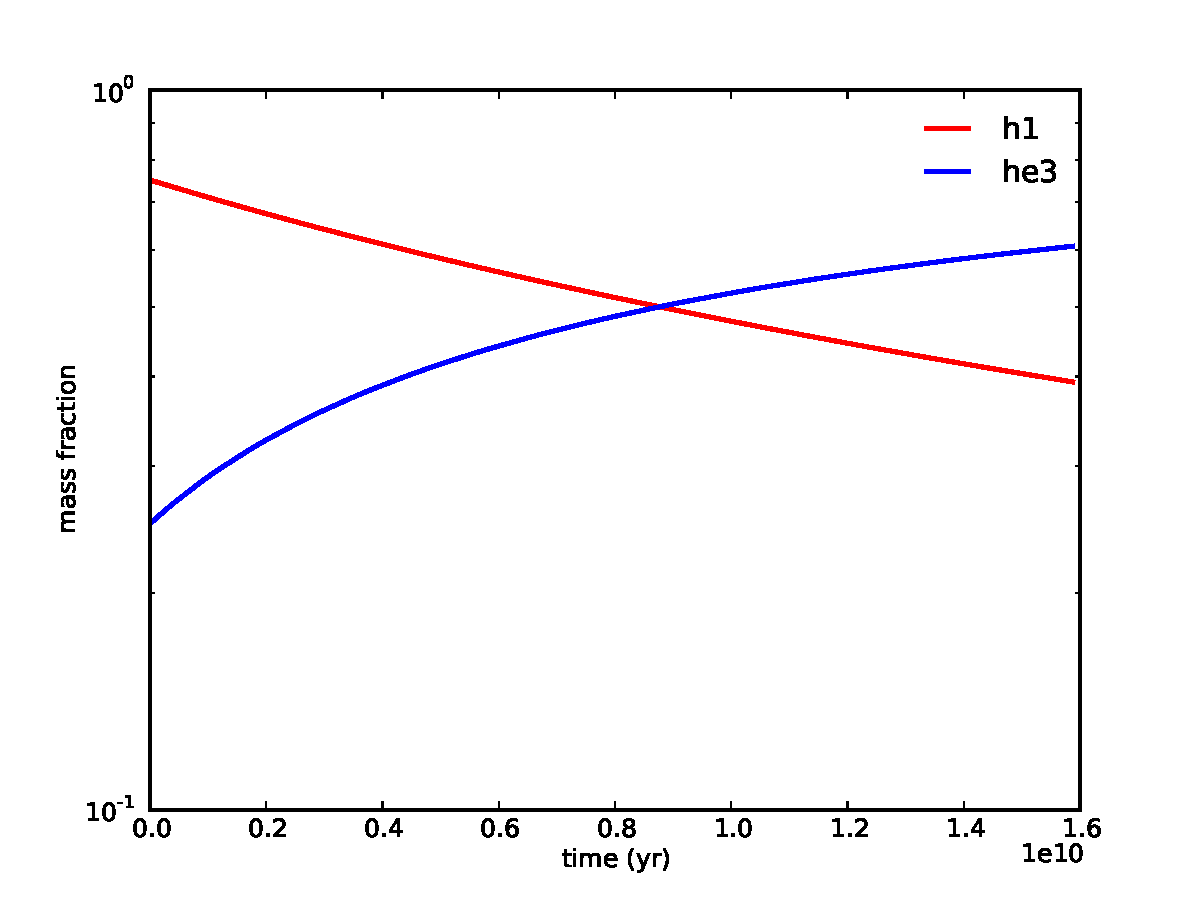
\includegraphics[width=5in]{T_1e7.pdf}
\end{center}
\caption{ \label{f:T_1e7}}
\end{figure}

\begin{figure}[!ht]
\begin{center}
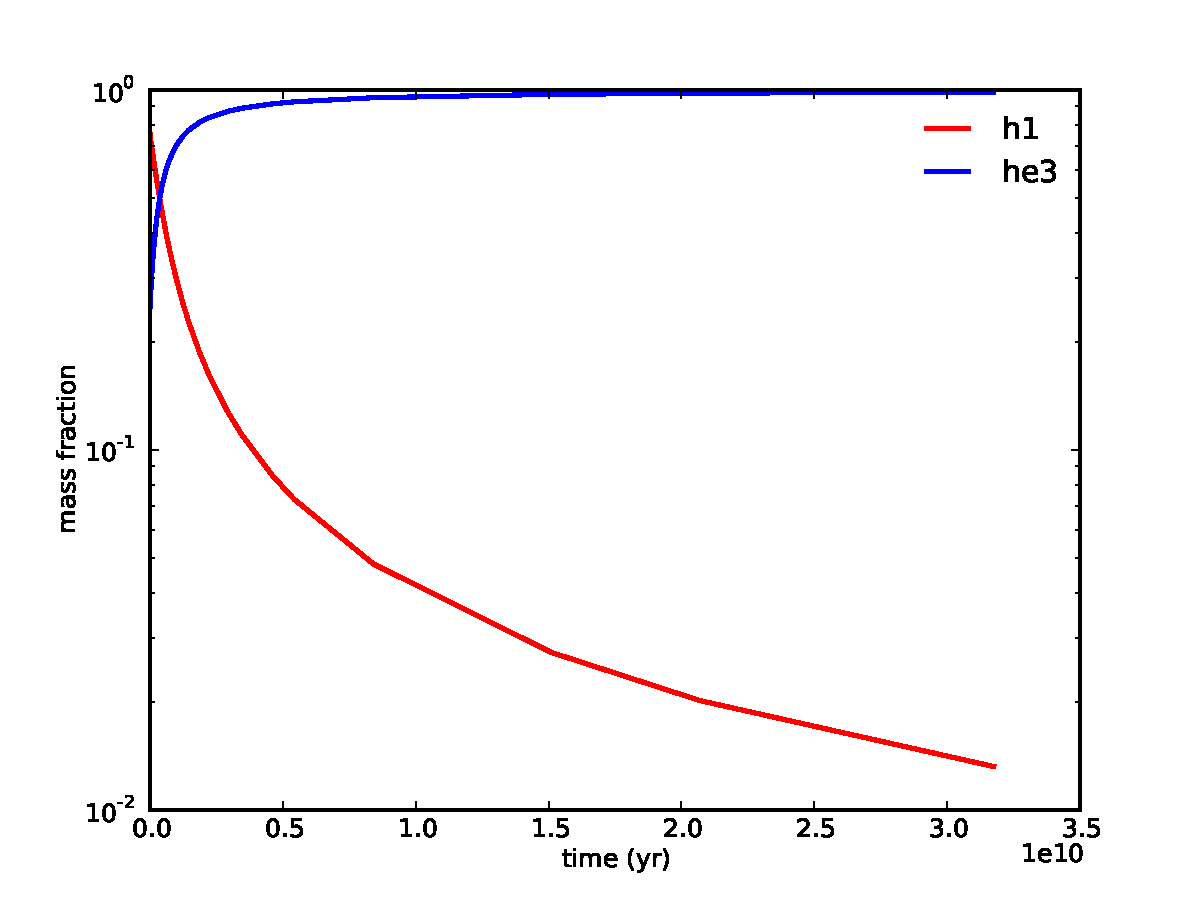
\includegraphics[width=5in]{T_2e7.pdf}
\end{center}
\caption{ \label{f:T_2e7}}
\end{figure}

\begin{figure}[!ht]
\begin{center}
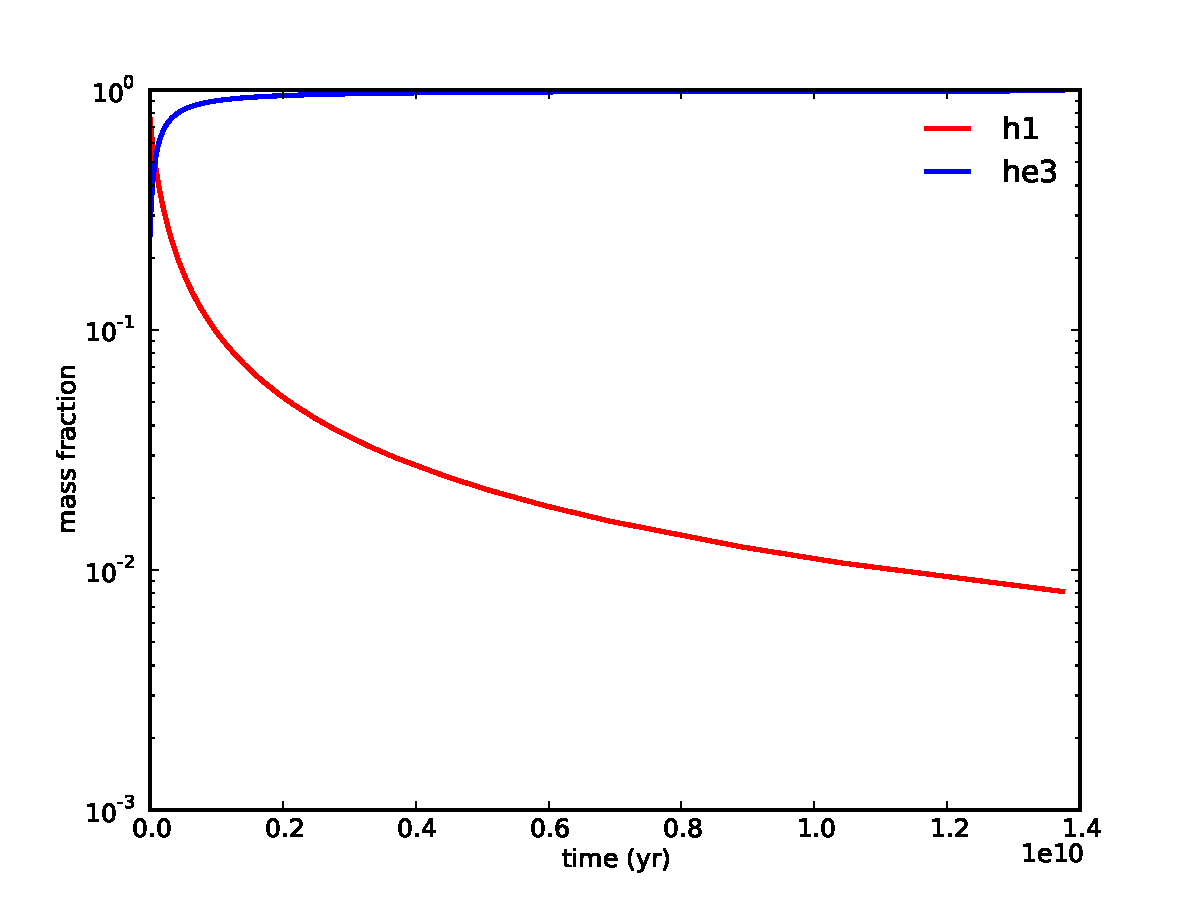
\includegraphics[width=5in]{T_3e7.pdf}
\end{center}
\caption{ \label{f:T_3e7}}
\end{figure}

The pp chain starts as follows:
\begin{equation}
^1_1{\rm H} + ^1_1{\rm H} \longrightarrow ^2_2{\rm He}
\end{equation}
\begin{equation}
^2_2{\rm He} \longrightarrow ^2_1{\rm D} + {\rm e}^+ + \nu_e
\end{equation}
The combination of these two reactions becomes:
\begin{equation}
^1_1{\rm H} + ^1_1{\rm H} \longrightarrow ^2_1{\rm D} + {\rm e}^+ + \nu_e + 0.42~{\rm MeV}
\label{eq:pp_1}
\end{equation}
We also have:
\begin{equation}
{\rm e}^- + {\rm e}^+ \longrightarrow 2\gamma + 1.02 MeV
\label{eq:pp_2}
\end{equation}
and
\begin{equation}
^2_1{\rm D} + ^1_1{\rm H} \longrightarrow ^3_2{\rm He} + \gamma + 5.49~{\rm MeV}.
\label{eq:pp_3}
\end{equation}
Then, for the pp I branch, 
\begin{equation}
^3_2{\rm He} + ^3_2{\rm He} \longrightarrow ^4_2{\rm He} + 2^1_1{\rm H} + 12.86~{\rm MeV}.
\label{eq:pp_4}
\end{equation}
We want to create a network using Equations \ref{eq:pp_1}, \ref{eq:pp_2}, \ref{eq:pp_3}, and \ref{eq:pp_4}.


%\bibliographystyle{apj2} 
%\bibliography{gal}

%\bibliography
\end{document}
